\chapter{Analys av punktmolnsregistrering}
\label{cha:indiv-report-karlsson}
\chapterprecis{\LARGE{---- Michael Karlsson ----}}


\section{Inledning}
\label{sec:introduction-karlsson}

%% Skriv här
I den här delen behandlas undersökningen av olika registreringsalgoritmer utförd av Michael Karlsson i samband med Kandidatprojektkursen TDDD96 samt de problem som projektgruppen stött på gällande registrering av punktmoln.

\subsection{Syfte}
\label{sec:purpose-karlsson}

%% Skriv här
Syftet med denna delen är att väga olika algoritmer mot varandra och undersöka hur väl de fungerade för det projekt som beskrivs i rapporten samt vilka problem gruppen hade med de olika algoritmer som testades. Gruppens tillvägagångssätt för val av algoritm undersöks också.


\subsection{Frågeställning}
\label{sec:issue-karlsson}

\begin{enumerate}
	\item Hur skapar man ett enhetligt punktmoln från enstaka bilder från en fast \newline avståndskamera?
	\item Hur gör man för att välja algoritm och hur resonerade gruppen när de valde ICP?	
\end{enumerate}

\subsection{Definitioner och förkortningar}
\label{sec:definitions-acronyms-karlsson}

Här listas de definitioner och förkortningar som används i kapitlet.

\begin{itemize}
	\item Point Cloud Library\cite{pcl_home} - Ett C++ bibliotek för hantering av punktmoln.
	\item PCL - Point Cloud Library.
	\item Iterative Closest Point - En algoritm för punktmolnsregistrering.
	\item ICP - Iterative Closest Point.
	\item JR-MPC - Joint Registration of Multiple Point Clouds
	\item SeqICP - SequentialICP
\end{itemize}


\subsection{Avgränsningar}
\label{sec:limits-karlsson}
Denna rapport kommer begränsas till hur processen fungerat med den hårdvara som vi blivit tilldelade. För registrering finns en ofantlig mängd algoritmer och tillvägagångssätt. Denna utredning kommer begränsas till de metoder som använts inom projektet. 


\section{Bakgrund}
\label{sec:background-karlsson}
I ett tidigt stadie av projektet upptäckte vi att en stor del skulle handla om att få registreringen att funka bra. Tidiga tester visade dessutom att meshningen, en annan del som tidigt verkade väldigt stor, som görs efter registreringen var förhållandevis enkel att utföra. Meshning innebär att man, utifrån det kompletta punktmolnet, skapar en vattentät 3D-modell. Jag blev intresserad efter att ha jobbat en del med tidiga försök till registrering och beslutade mig för att djupdyka i ämnet.


\section{Teori}
\label{sec:theory-karlsson}

När man vill återskapa fysiska objekt digitalt fastnar man oftast i att det inte finns några bra verktyg för att läsa in tredimensionella objekt. Man behöver då ta flera bilder av objektet från olika vinklar för att kunna sammanfoga dessa till det fulla objektet. Det finns många metoder för detta, exempelvis Kinect Fusion. Den metod vi använt oss av har dock bestått av en avståndskamera på en linjärenhet med objektet monterat på ett rotationsbord med 2 rotationsaxlar. Med hjälp av detta rotationsbord kan men förhållandevis enkelt se hela objektet från en fast punkt. Dessa punktmoln har vi haft som moln att enhetligt registrera till en komplett representation av objektet som skannats.


\subsection{Registrering}
\label{sec:registrering-karlsson}

Registrering är den generella metoden att sätta ihop två eller flera punktmoln till ett koordinatsystem med all information från indatan. Det finns väldigt många olika algoritmer för att utföra detta såsom till exempel ICP, \textit{Iterative Closest Point} eller GMMReg. De flesta tillgängliga algoritmer har någon form av svaghet eller nackdel. Till exempel så lider ICP av så kallad \textit{felutbredning} och JR-MPC, \textit{Joint Registration of Multiple Point Clouds}, lider av längre körtid.[]

\subsection{Kinect Fusion}

Kinect fusion använder sig av Microsofts egna avstånds- och RGB-kamera, Kinect, för att mappa upp ett 3D objekt i den verkliga världen. Avståndskameran mäter upp punktmolnet för scenen framför den samtidigt som en synkroniserad RGB-kamera ger färgdata till varje punkt. 
Varje punktmoln som Kinect kameran skickar består av ca 307 000 punkter. Det kan jämföras med hårdvaran som vi använt oss av där maximala antalet punkter i en skanning är ca 786 000 punkter. De punktmoln som vi arbetat med har dock generellt innehållit ca 30-60 000 punkter efter filtrering av skräpdata.

\section{Metod}
\label{sec:method-karlsson}

Här presenteras metoden som använts för att besvara frågeställningarna i kapitlet. De är uppdelade i hur arbetet för att besvara frågorna gick till i förstudien för rapporten samt under utvecklingsarbetet.

\subsection{Förstudie}
Initialt gjordes en litteraturstudie för att hitta information om hur man går till väga för att registrera punktmoln.  PCL ger många handledningsexempel med exempelkod som blev utgångspunkten för utbildningen om registrering i gruppen. PCL ger också en bra sammanfattning men utöver det saknas relevanta källor. Då utredningen är begränsad till framförallt ICP och JR-MPC begränsas antalet källor ytterligare. Det finns enormt många varianter av ICP, såsom SeqICP, Point-to-Plane ICP Point-to-Point ICP m.fl. Den variant som utvärderas här är den som implementeras av PCL, Point-to-Point. 

JR-MPC är resultatet av en forskningsstudie som tagit fram algoritmen och därmed finns enbart den källa som används här för den algoritmen. Det finns snarlika algoritmer med enbart sina forskningsdokument som källa men dessa kommer alltså inte behandlas här.

\subsection{Utvecklingsfas}
Ett experiment utfördes för att jämföra ICP och JR-MPC. Testet gick ut på att registrera en uppsättning om 36 punktmoln. Vart och ett av dessa punktmoln var en skanning av kyrkan, se fig \ref{fig:karlsson-single_scan-church}, där kyrkan skannats och roterats 10 grader efter varje skanning. 

\begin{figure}[H]
	\centering
	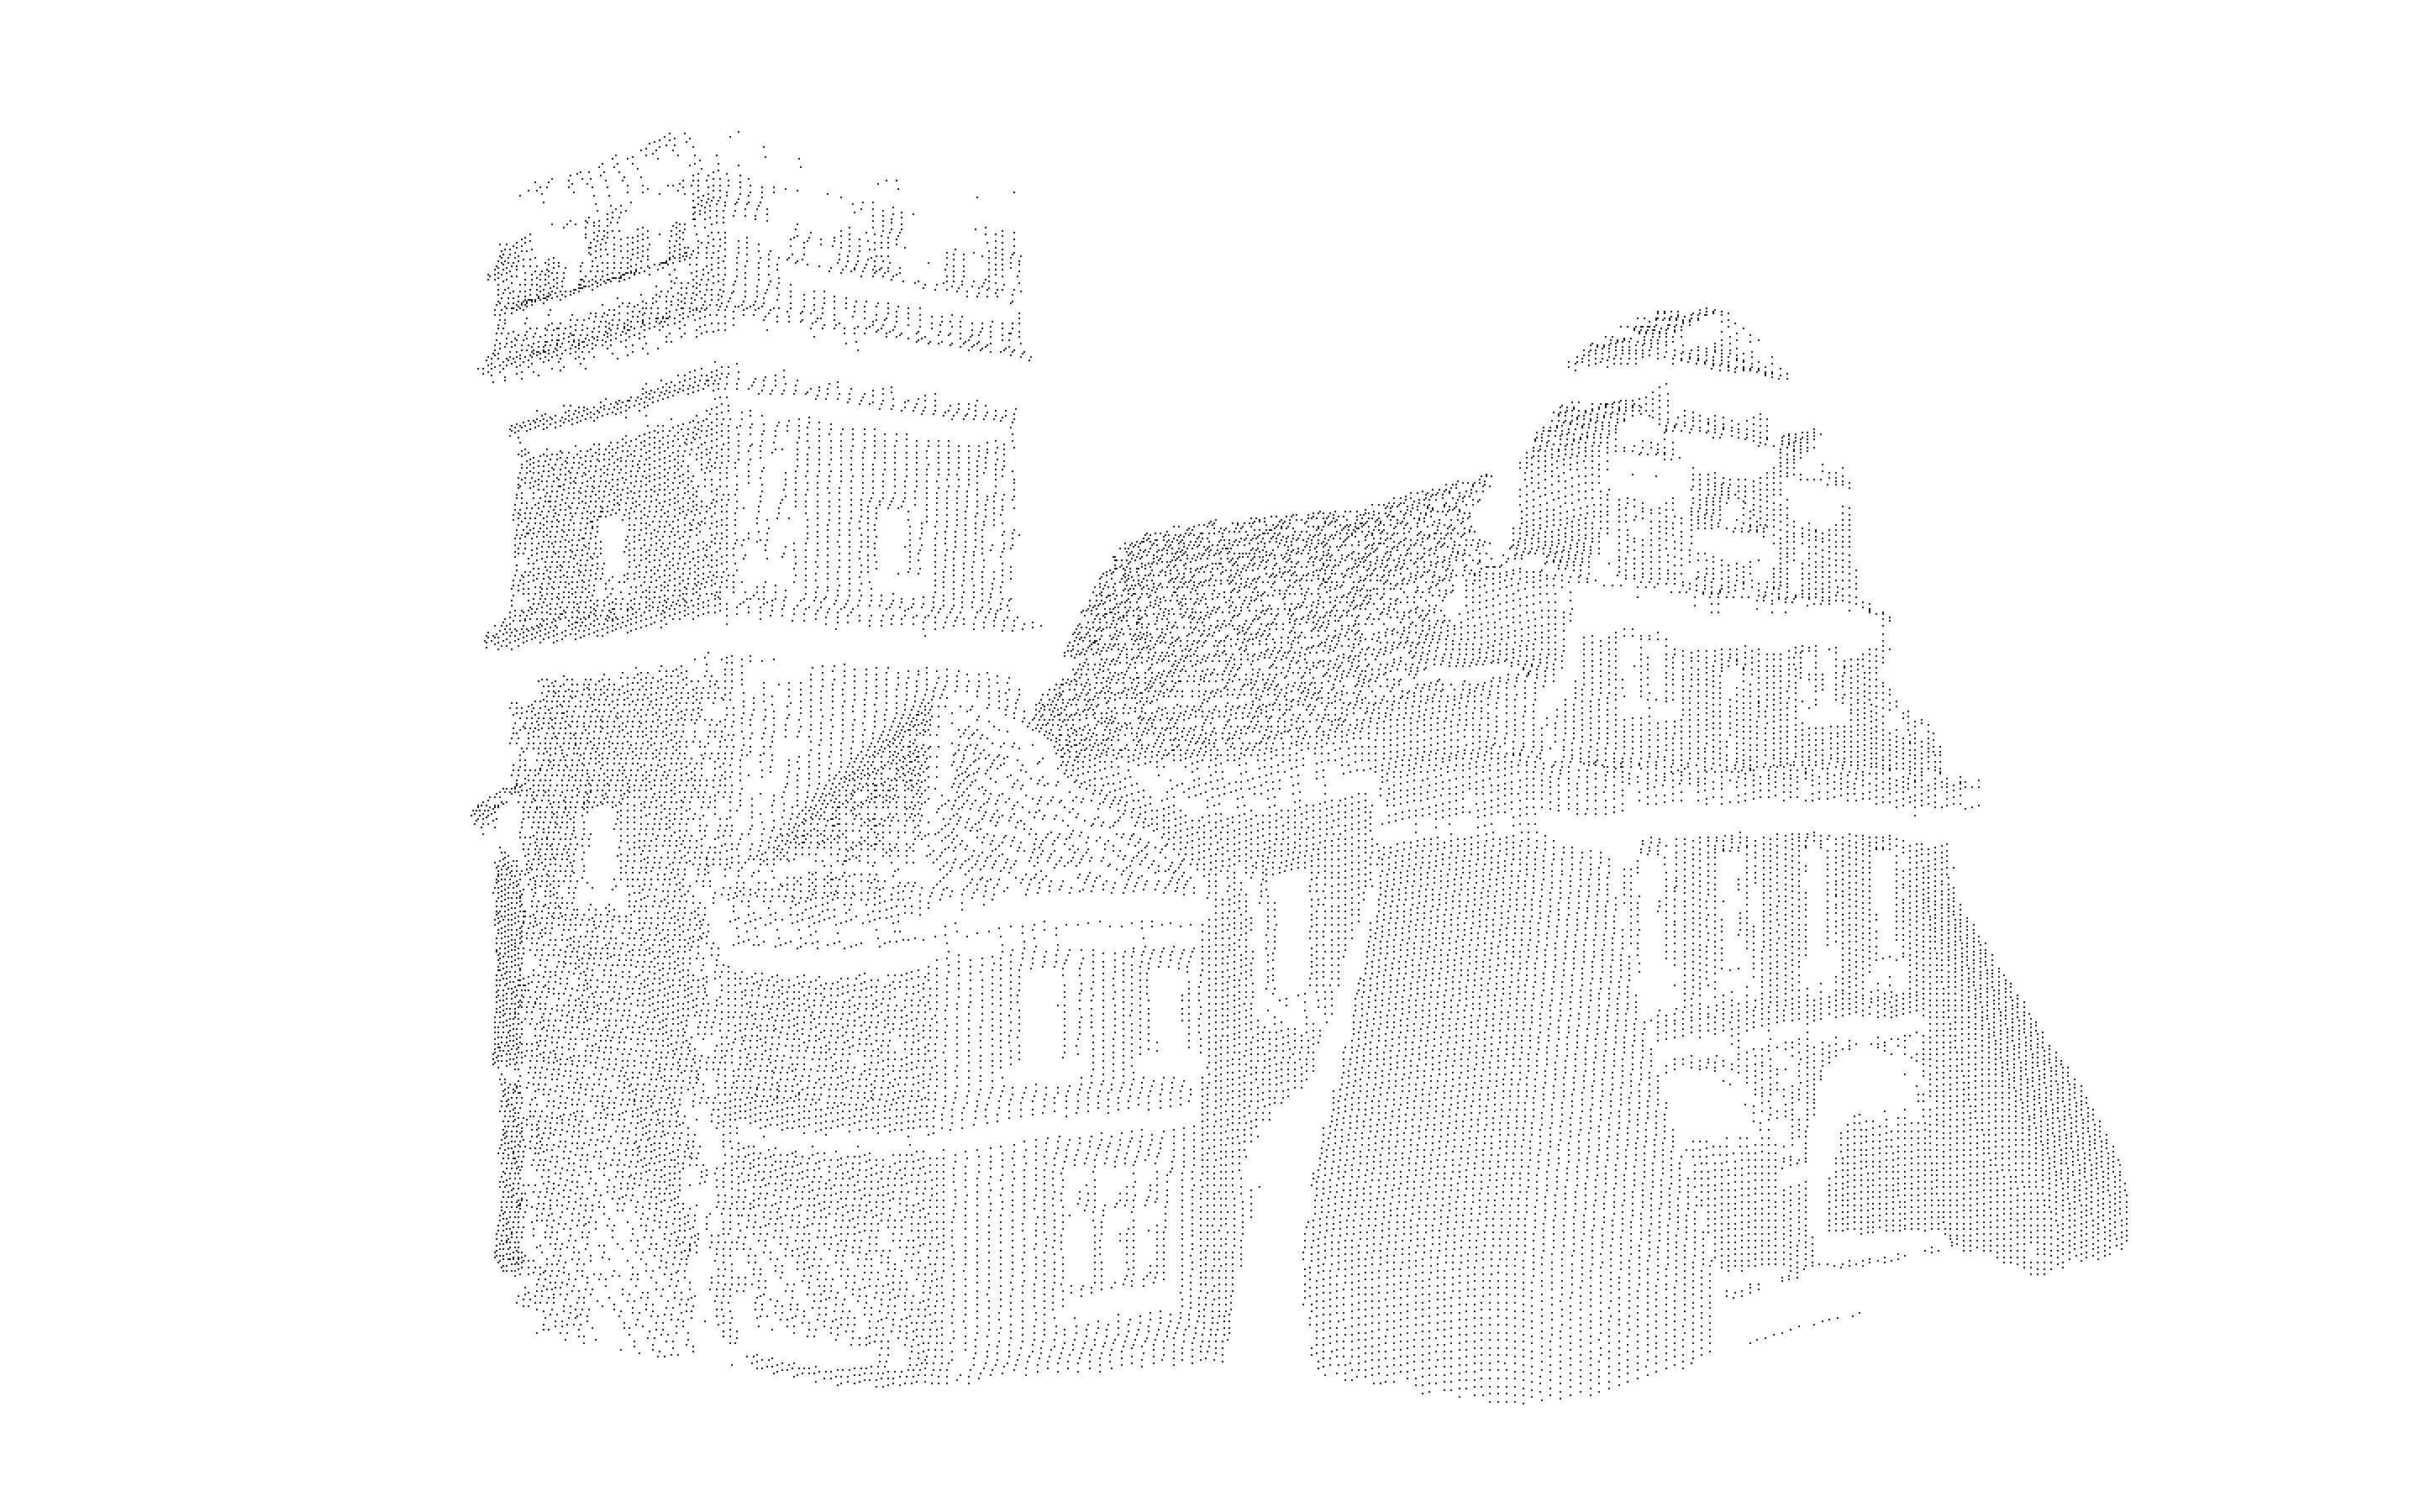
\includegraphics[width=100mm]{figures/icke_komplett_moln_kyrka.png}
	\caption{Ett icke komplett punktmoln som representerar en del av en kyrka.}
	\label{fig:karlsson-single_scan-church}
\end{figure}


\section{Resultat}
\label{sec:results-karlsson}

%% Skriv här

% Resultatet av experiment 1 ses i fig XX samt fig XX. 
% Som vi kan se så har ICP lyckats relativt bra, _stegvis bilder_ se fig XX. 
Vi började med att införskaffa oss en uppsättning punktmoln på objektet och försökte med den exempelkod vi hittat sätta ihop punktmolnen. De första objektet vi började testa med var en porslinskyrka p.g.a. att det var det enda vi hade att tillgå. Efter ett par veckor fick vi en låda med träklossar som vi började arbeta med och som blev gruppens primära mål att registrera då dessa rekommenderades av kund som lättare objekt. Den primära algoritm vi använde var ICP. 

Valet av ICP var initialt enbart baserat på att det var den algoritm vi hittade först samt den som vi fick tag på exempelkod för. Vi gjorde dock vissa begränsade tester med JR-MPC som rekommenderades av kunden CVL. Då JR-MPC inte vid tidpunkten gav bättre resultat än den metod som användes samt betydligt mer manuellt arbete för att kunna köra algoritmen så lades arbetet med JR-MPC på is. Mer fokus lades på att jobba vidare med ICP och ungefär halvvägs in i projektet hade vi en algoritm som funkade bra för de första 13 punktmolnen. Senare punktmoln hamnade mer och mer fel tills felet blev markant runt 19 registrerade punktmoln. 


\subsection{ICP}
ICP är en optimeringsalgoritm som försöker minimera det totala avståndet från varje punkt i ursprungsmolnet till varje punkt i målmolnet. Det ger algoritmen en tidskomplexitet $ \mathit{O(n*m)} $ där $ \mathit{n} $ är antalet punkter i ursprungsmolnet och $ \mathit{m} $ är antalet punkter i målmolnet. Som tidigare nämnt så har ICP ett ursprungsmoln som aldrig ändras samt ett målmoln som försöker passas in så det stämmer överens med ursprungsmolnet. 

ICP har ett antal parametrar för att bestämma hur registreringen ska gå till. De parametrar som undersökts inom gruppen listas nedan och förklaras mer ingående nedan.
\begin{itemize}
	\item Max Iterations
	\item Transformation Epsilon
	\item Max Correspondence Distance
	\item RANSAC Outlier Rejection Threshold
	\item Euclidean Fitness Epsilon
\end{itemize}
\textbf{Max Iterations} anger hur många registrerings\-iterationer som algoritmen får utföra innan den tvingas avsluta.\\
\textbf{Transformation Epsilon} avgör hur stor förflyttning algoritmen får göra på målmolnet inom en iteration.\\
\textbf{Max Correspondence Distance} anger hur stort avståndet från en punkt i ursprungsmolnet till motsvarande punkt i målmolnet får vara. Är avståndet större än detta kommer algoritmen ignorera punkten i målmolnet vid registreringsförsöket.\\
\textbf{RANSAC Outlier Rejection Threshold} anger hur stort avstånd som en punkt tillåts existera från den antagna matematiska modellen för att användas i registreringen. RANSAC, \textit{Random Sample Consensus} är en metod för att avgöra om en punkt följer det matematiska mönster som algoritmen letar efter.\\
\textbf{Euclidean Fitness Epsilon} representerar det fel som accepteras. Är skillnaden i felet mellan två iterationer mindre än det här kommer algoritmen avsluta.

\subsection{JR-MPC}
JR-MPC använder så kallade GMM, \textit{Gaussian Mixture Model}, för att registrera objektet. Exakt hur matematiken bakom algoritmen ser ut och fungerar är utanför omfattningen av denna rapport men grundläggande principer följer. GMM är en sannolikhetsmodell som används för att lista sannolikheten att ett kluster av punkter i punktmolnet är en del av objektet som ska registreras, detta motsvarar RANSAC filtreringen som görs i ICP. Själva registreringen görs genom en förväntad villkorlig maximering, ECM, \textit{Expectation Conditional Maximization}. För fördjupning om ECM hänvisas till \cite{}.

\subsection{3DCopy metoden}
Under utvecklingsarbetet och problemfaser med registreringen planerade gruppen om och försökte med en annan lösningsmetod till registreringsproblemet. Under detta arbete hade gruppen som fokus att lyckas med de objekt som, enligt kravspecifikation, definierades som "lätta". Dessa objekt bestod av en träkloss formad som en kub samt en "träbro", se fig \ref{fig:foto_church}. Då registreringsalgoritmerna som använts helt ignorerar den kända datan om hur mycket rotation som skett mellan varje skanning så blev det fokus för våran metod. Genom att göra flera skanningar över en rotation på 90 grader kan den plattaste skanningen hittas. Därifrån tas fyra skanningar av objektet, utan lutning, med 90 grader mellan varje skanning och resultatet av dessa blir varje kardinal sida av objektet. Vid vidareutveckling av algoritmen hade dessutom en sista skanning gjorts för att få med ovansidan av objektet. Dessa kan därefter registreras på ett virtuellt objekt där varje sida ges av en motsvarande skanning. Principiellt så tänker vi oss att varje skannad sida av ett objekt "klistras på", på ett virtuellt objekt skapat med liknande dimensioner. 

\begin{figure}[H]
	\centering
	\includegraphics[width=70mm]{figures/Foto_church.png}
	\caption{Porslinskyrkan som använts för test av skanning och registrering}
	\label{fig:foto_church}
\end{figure}

\subsection{ICP vs. JR-MPC}

Vid jämförande av ICP så finns ett par signifikanta skillnader. 

På grund av att ICP är en mer rudimentär algoritm än JR-MPC så blir den också lättare att implementera. JR-MPC bygger på mer avancerad matematik som måste förstås för att kunna implementera den.

Enligt \cite{Evangelidis-ECCV-2014} så är ICP en aning snabbare än JR-MPC vilket dock inte har replikerats i projektets begränsade tester. Då tidsåtgången för komplett registrering av 36 punktmoln med ICP är i närheten av 3 timmar så har inte någon ingående studie gjorts. 

Som nämndes i \ref{sec:registrering-karlsson} så påverkas algoritmerna väldigt olika av fel, såsom till exempel avrundningsfel som är oundvikligt med flyttal. Då ICP\footnote{Notera att detta endast gäller vissa ICP algoritmer} bara tillåter parvis registrering, dvs att ett punktmoln registreras med ett annat kommer dessa avrundningsfel växa och bli större ju fler punktmoln som registreras. Dessutom sparas i våran implementation det parvis registrerade punktmolnet som ett färdigt oföränderligt punktmoln och ev avrundningsfel kan bara elimineras genom att köra algoritmen igen med andra parametrar.

\subsection{Resultat av Experiment 1}

Resultatet av experimentet som utfördes presenteras här med ett antal bilder.  

\begin{figure}[H]
	\centering
	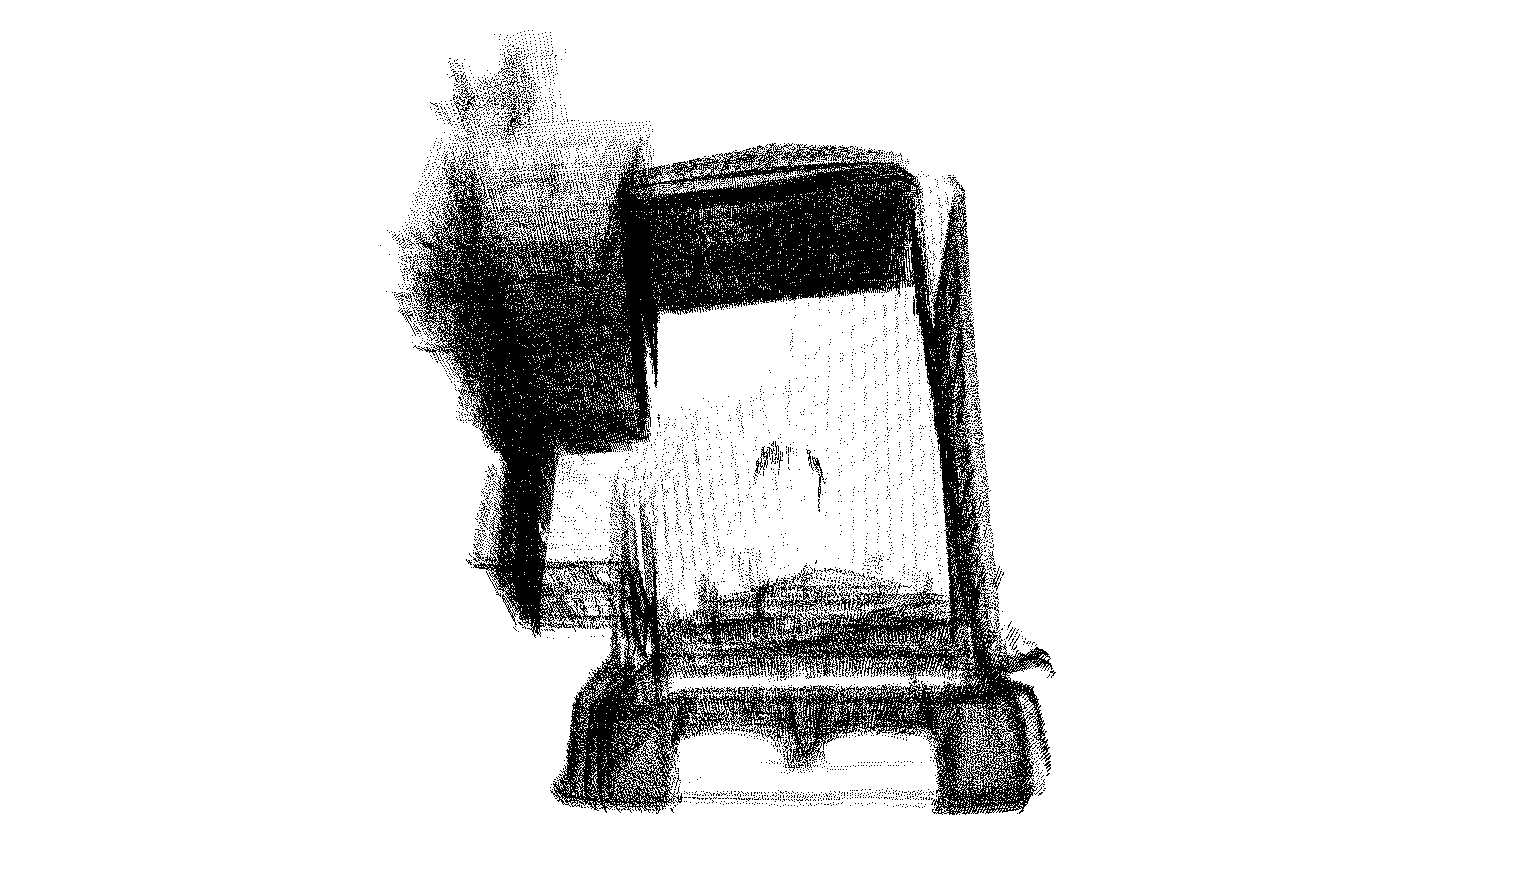
\includegraphics[width=65mm]{figures/first_registered_church.png}
	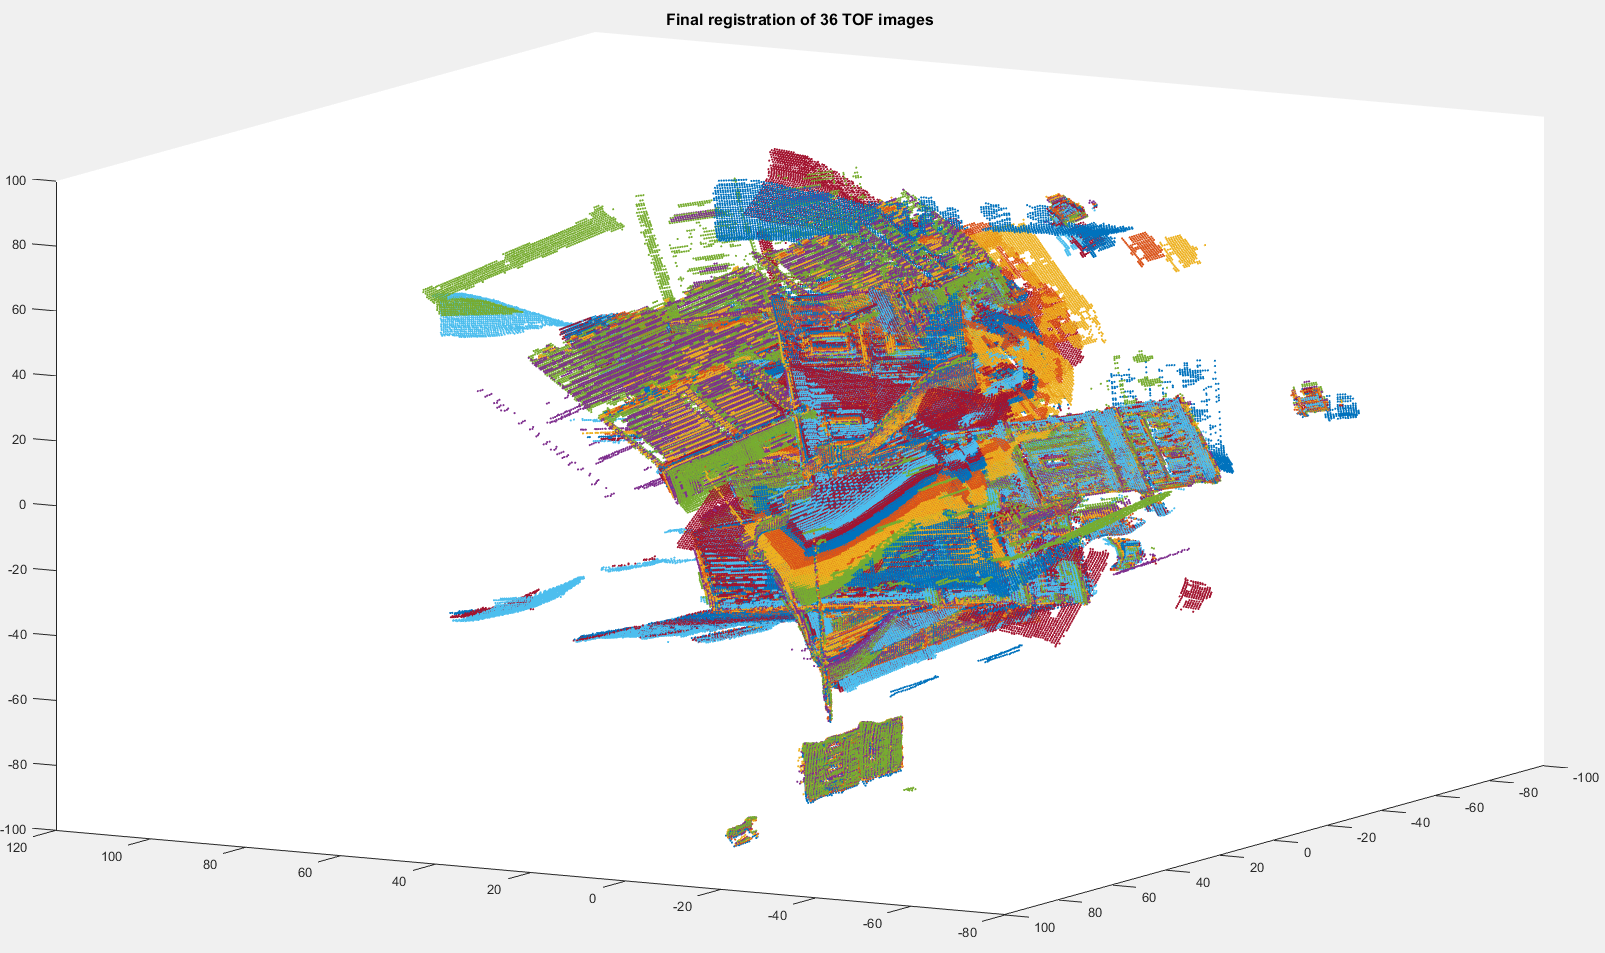
\includegraphics[width=65mm]{figures/JRMPC_result.png}
	\caption{Till vänster: Resultat från registrering med ICP, Till höger: Resultat från registrering med JR-MPC}
	\label{fig:icp_vs_jrmpc_result}
\end{figure}

Nedan i fig \ref{fig:registrered_church_serie} ses från övre vänstra till nedre högra bilden delresultatet av 12, 13, 18, 19 samt 20 punktmoln extraherat från en och samma körning. Notera till exempel resultatet för 20 punktmoln där man tydligt i främre vänstra hörnet på kyrkan ser dubbla hörn. Det här kommer av att punktmolnen som registreras, enligt ICP, ligger i varandra vid starten. Efter 12 punktmoln behöver därmed nästa moln roteras 130 grader och sannolikheten för ett falskt optimum ökar.
\begin{figure}[H]
	\centering
	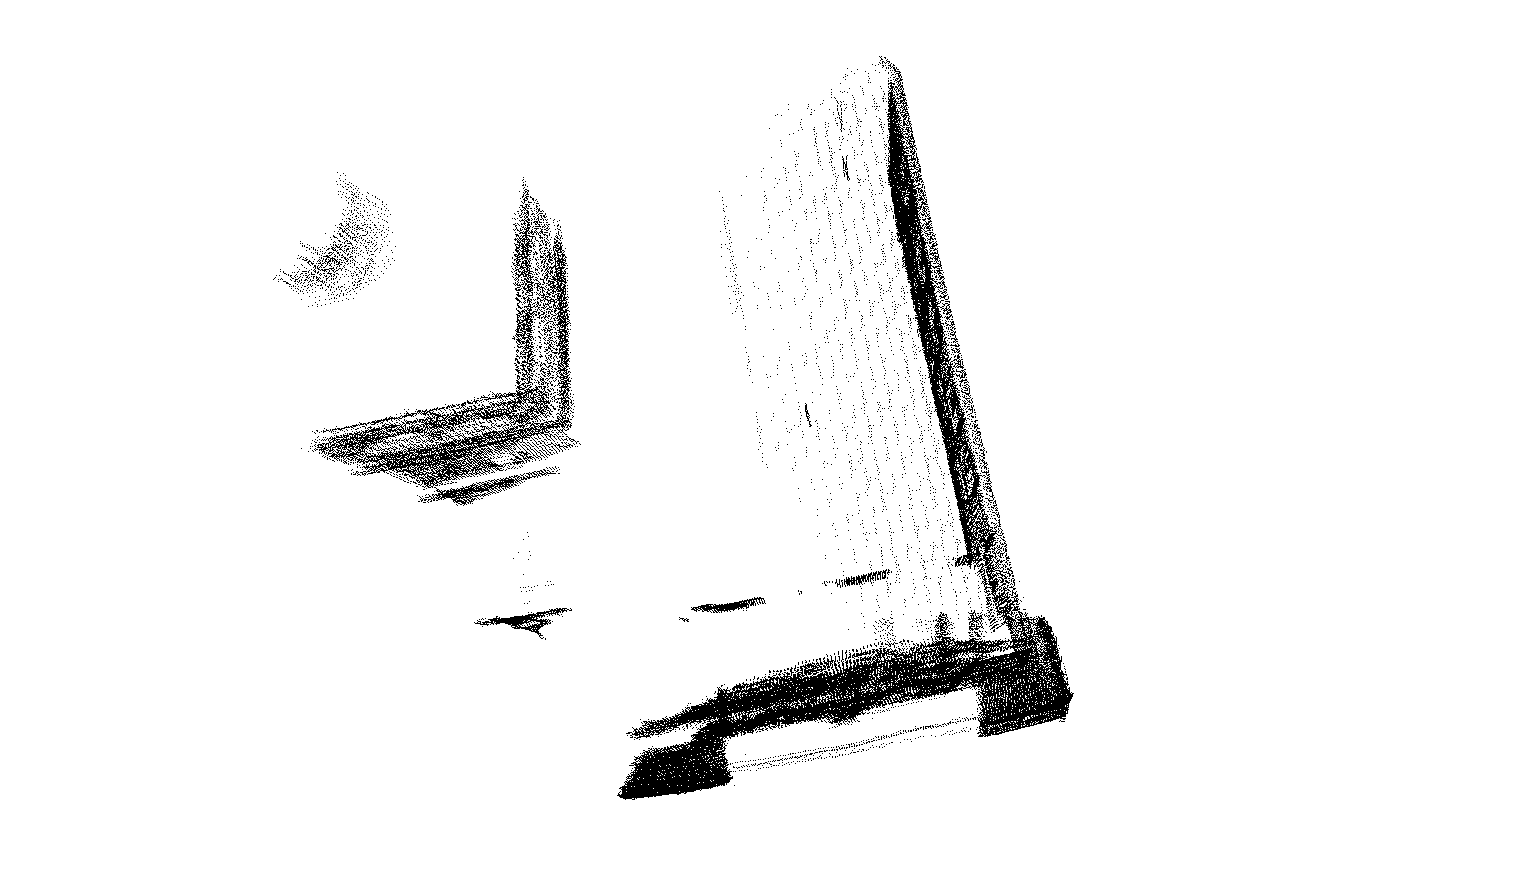
\includegraphics[width=45mm]{figures/12_pc.png}
	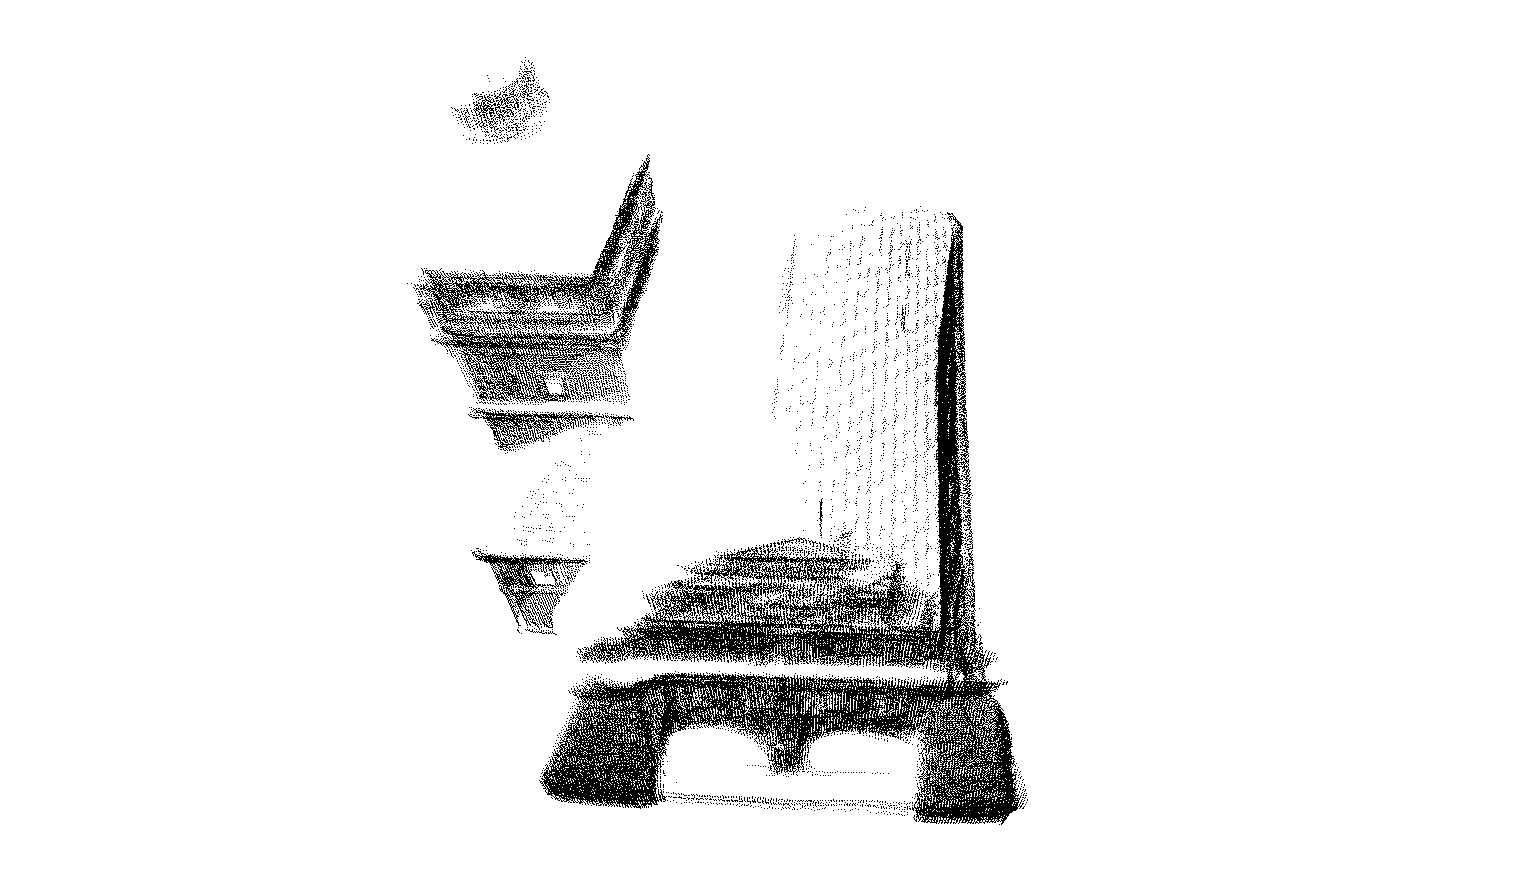
\includegraphics[width=45mm]{figures/13_pc.png}
	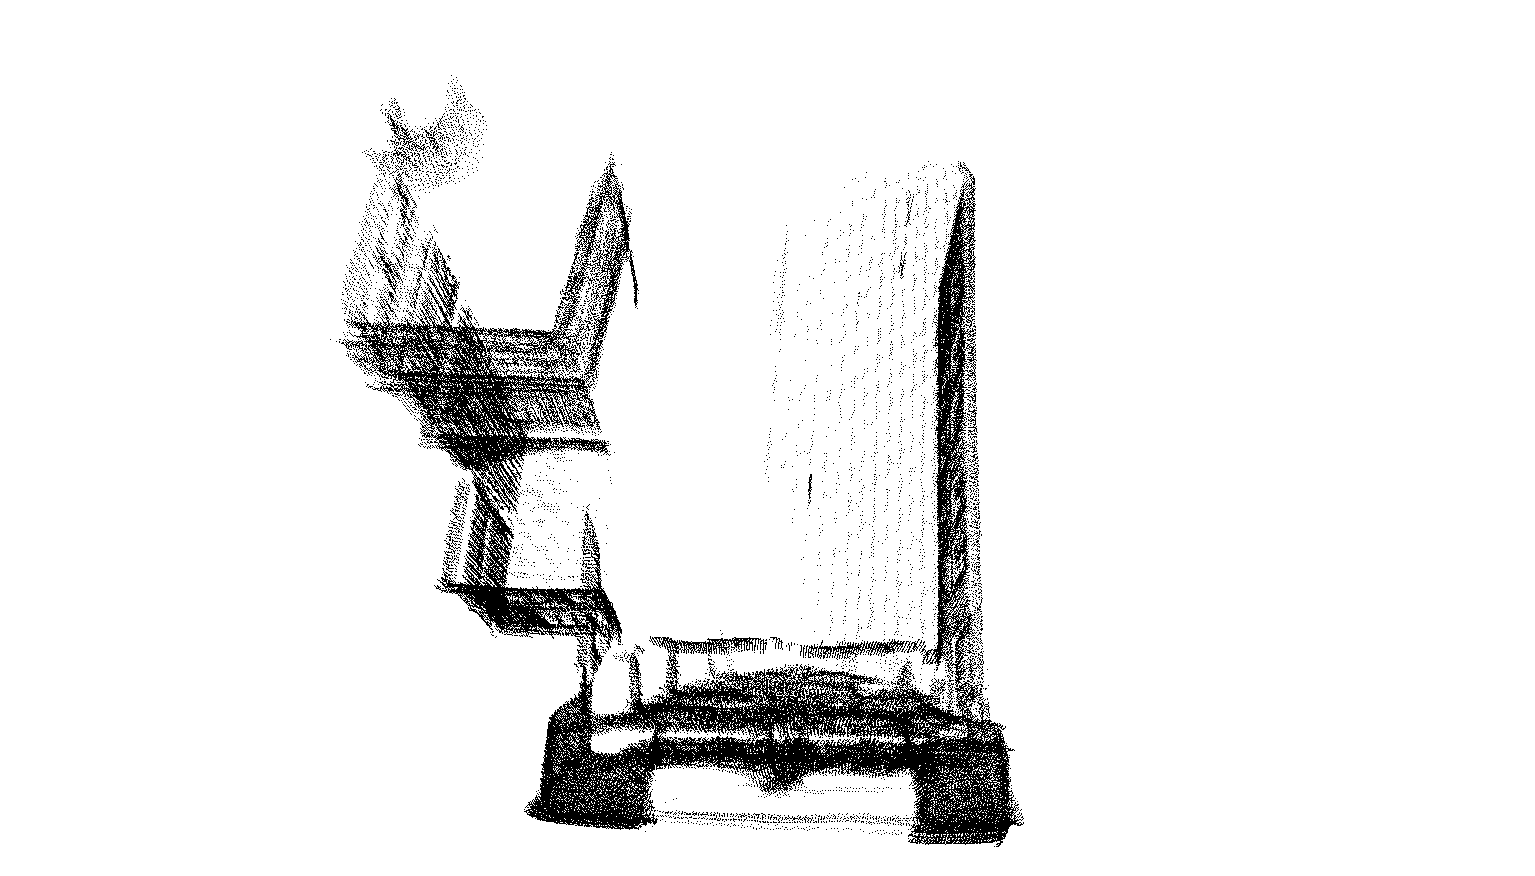
\includegraphics[width=45mm]{figures/18_pc.png}
	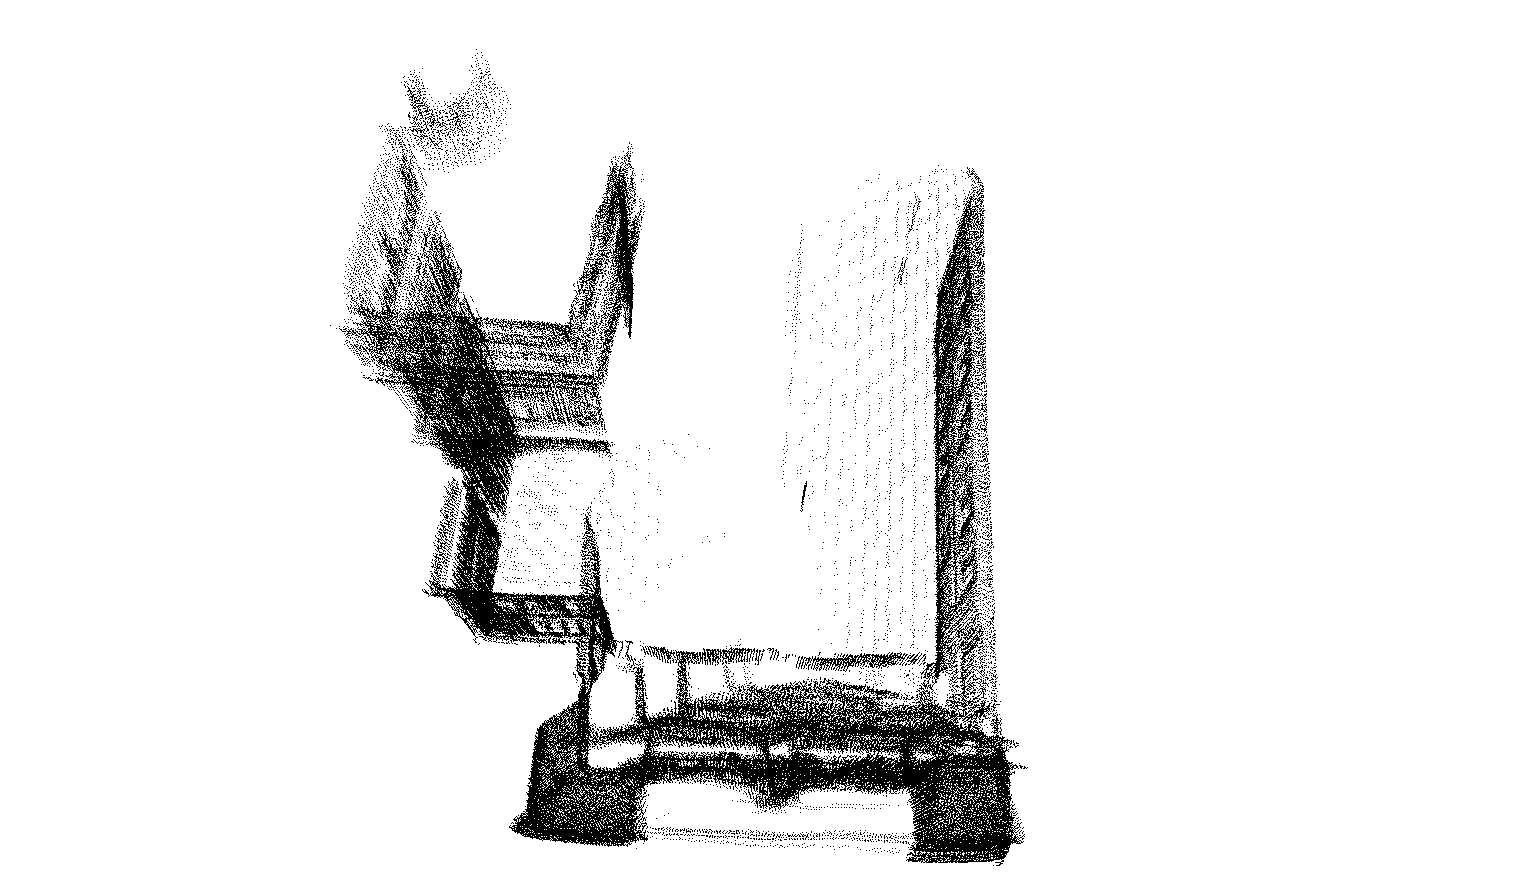
\includegraphics[width=45mm]{figures/19_pc.png}
	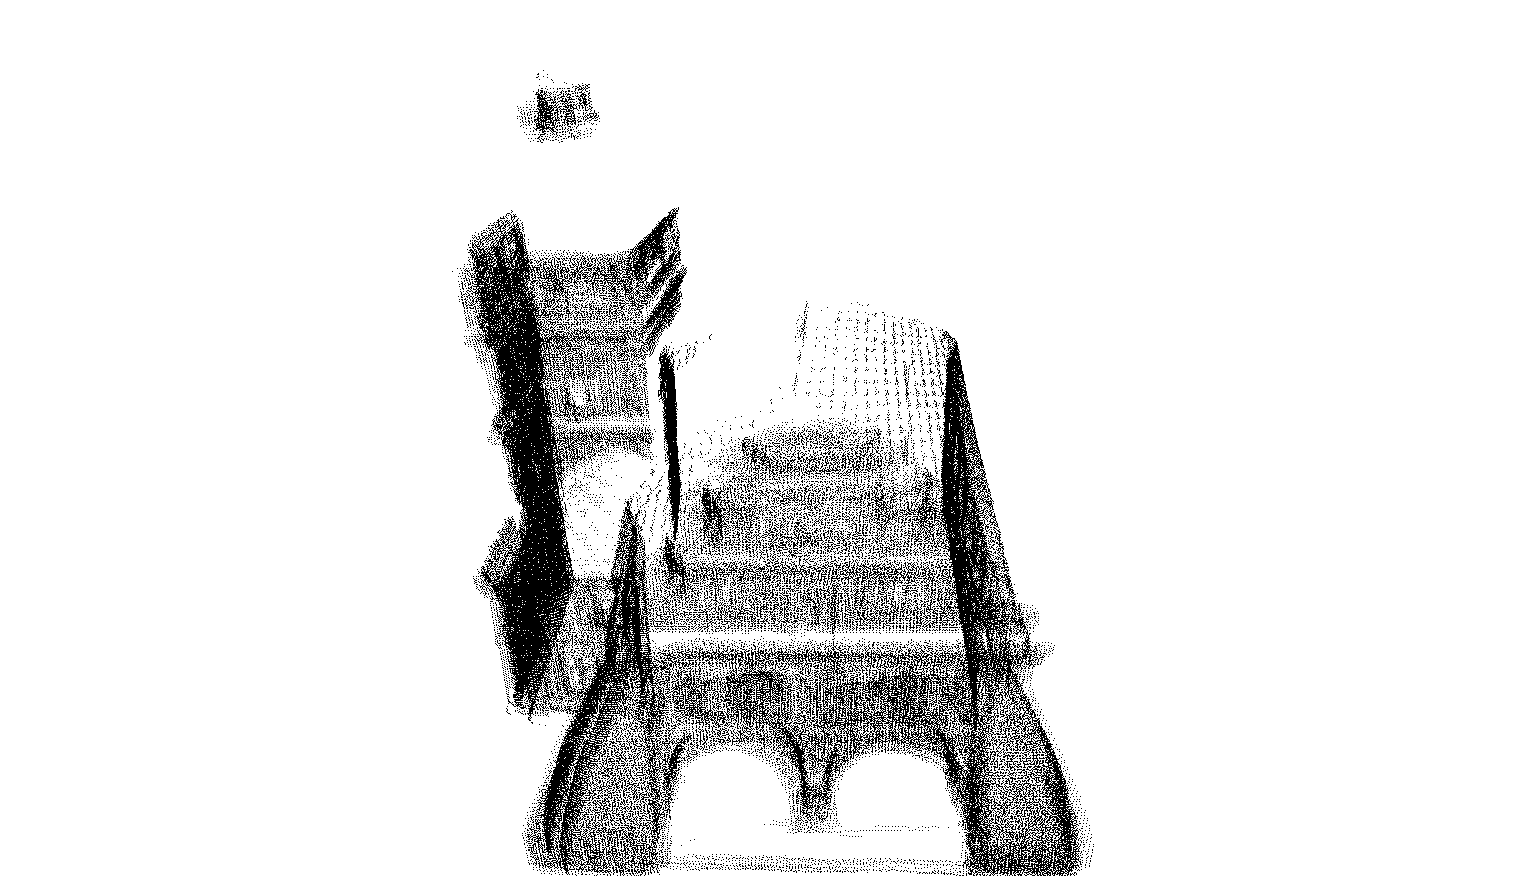
\includegraphics[width=45mm]{figures/20_pc.png}
	\caption{Serie av delresultat från registrering med ICP}
	\label{fig:registrered_church_serie}
\end{figure}

\section{Diskussion}
\label{sec:discussion-karlsson}

Den implementation av JRMPC som vi fick tag på funkade väldigt dåligt för den typ av data som vi hade. På grund av att algoritmen är väldigt komplicerad och inte tillräckligt dokumenterad för att vi skulle kunna hitta parametrar att ändra på för att förbättra resultatet så beslutades att ICP skulle användas och optimeras.

3DCopy använder sig av \textit{Max Iterations}, \textit{Transformation Epsilon} samt \textit{Max correspondence distance}. Då PCLs standardvärden för \textit{RANSAC outlier rejection threshold} samt \textit{Euclidean fitness epsilon} funkade bra för gruppen användes dessa och de går inte ändra i 3DCopy. Det är dock väldigt lätt att lägga in stöd för det om programmet skulle vidareutvecklas.

\subsection{Diskussion om Metod}



\subsection{Diskussion om Resultat}

\subsubsection{Diskussion om Experiment 1}



\section{Slutsatser}
\label{sec:conclusions-karlsson}

%% Skriv här

%%%%%%%%%%%%%%%%%%%%%%%%%%%%%%%%%%%%%%%%%%%%%%%%%%%%%%%%%%%%%%%%%%%%%%
%%% karlsson-report.tex ends here
